\documentclass[12pt,a4paper,english,twoside]{article}

\usepackage[T1]{fontenc}
\usepackage[utf8]{inputenc}
\usepackage[english]{babel}
\usepackage{amsmath}
\usepackage{amsfonts}
\usepackage{mathtools}
\usepackage{fancyhdr}
\usepackage{graphicx}
\usepackage{hyperref}
\usepackage{tikz}
\usepackage{listings}
\usepackage{float}
\usepackage{csvsimple}
\usepackage{pgfplots}

\usepackage{sty/pgf-umlsd}

\usetikzlibrary{arrows,calc,shapes,positioning,chains,decorations.pathreplacing}

% Header and Footer Style
\fancyhead{}
\fancyhead[R]{\slshape Patrick Steinhardt}
\fancyhead[L]{\slshape\nouppercase{\rightmark}}
\fancyfoot{}
\fancyfoot[C]{\thepage}
\renewcommand{\headrulewidth}{0pt}
\renewcommand{\sectionmark}[1]{\markright{\thesection\ #1}}

% No identation
\setlength\headheight{15pt}
\setlength\parindent{0pt}

% Break after each section
\let\stdsection\section
\newcommand{\bigparskip}{\vspace{12pt}}

\bibliographystyle{alpha}

\widowpenalty10000
\clubpenalty10000

\lstset{language=C}
\lstset{captionpos=b}

% Titel and author
\title{A Protocol for Connecting Distributed Resources}
\author{Patrick Steinhardt}
\date{Berlin, \today}

\begin{document}

    \pagenumbering{gobble}
    \begin{titlepage}
    \makeatletter
    \begin{center}
        \vspace*{2cm}

        {\Large \@title}
        \vspace*{1cm}

        {\large \@author}

        \vspace*{\fill}

            Submitted to the Department of Computer Science\\
            of the Freie Universität Berlin\\
            in partial fulfillment\\
            of the requirements for the degree of\\
            Master of Science

        \vspace*{\fill}

        \@date
        \vspace*{2cm}
    \end{center}

    \makeatother
\end{titlepage}

% vim: ft=tex tw=0

    \vspace*{\fill}


\begin{minipage}{0.7\textwidth}
    This work is licensed under the Creative Commons Attribution-ShareAlike 4.0 International License.
    To view a copy of this license, visit \url{http://creativecommons.org/licenses/by-sa/4.0/}.
\end{minipage}
\hfill
\begin{minipage}{0.25\textwidth}
    \includegraphics[width=\textwidth]{resources/by-sa.eps}
\end{minipage}

\pagebreak

% vim: tw=0

    \subsection*{Affirmation}

I hereby declare to have written this thesis on my own.
I have used no other literature and resources than the ones referenced.
All text passages that are literal or logical copies from other publications have been marked accordingly.
All figures and pictures have been created by me or their sources are referenced accordingly.
This thesis has not been submitted in the same or a similar version to any other examination board.

\vspace{4em}

\begin{tabular}{c}
    \rule{7cm}{1pt}\\
    \makeatletter\@date\makeatother
\end{tabular}

% vim: ft=sh tw=0


    \clearpage

    \pagenumbering{Roman}
    \tableofcontents
    \clearpage
    \listoffigures
    \clearpage
    \lstlistoflistings
    \clearpage

    \pagestyle{fancy}
    \pagenumbering{arabic}
    \setcounter{page}{1}

    \section{Introduction}

In recent years it has become obvious that the power of global adversaries which are able to attack the information technologies infrastructure in significant ways is much greater than many have thought.
The most important sources indicating the vast capabilities of foreign intelligence services like the NSA or GCHQ are documents leaked by Edward Snowden, starting in 2013 (SOURCE).
Those documents draw a picture of a global surveillance network built primarily by the National Security Agency which is able to intercept, collect and analyze a significant portion of the global communications network.

But besides acting on the layer of informations flowing through cables, these agencies quite regularly act on the physical layer, as well.
The agencies have the ability to intercept hardware ordered by certain individuals and modify it such that it is possible to monitor these devices withouth the target knowing.
This may include tampering with device firmware such that certain programs may collect and dispatch ongoing events in the hardware system or attaching additional devices like microchips to the device.
Nowadays it is next to impossible to detect those modifications when the individual is not aware that he might be spied upon.

The latter scenario makes clear an important design flaw in modern personal computing systems.
That is, many devices enjoy unrestrained access to the complete architecture, including main memory and other system busses, making it trivial for hardware to monitor what is going on in a system.
As such, we do have to trust every connected hardware device like e.g. graphics cards to not include hostile components and thus compromise our system.

Despite the security aspect there is also the aspect of malfunctioning devices.
When device firmware is being buggy it is possible that the malfunctioning device may corrupt the system's state and thus lead to the system malbehaving or crashing.
\\\\
In this thesis we will develop a countermeasure to the ability of hardware devices having access to the full system.
Instead of directly connecting untrusted hardware devices to the busses, we will develop a protocol such that we are able to connect devices via a networking interface with the system.
As such the only interface that is used to connect to systems is the networking interface card.

As such we are now able to build a minimal system with only the most important devices like the CPU, main memory and the networking interface card.
Every other extension to the system will then communicate via a device-type specific protocols that may be verified on the host system.

In order to get a working system we require a service that has to handle events when new devices are connected or disconnected to the system.
This matchmaking service will have to determine if the connected device is supported and associate the respective drivers to the device.
Furthermore there might be several security concerns which will need to be handled by the matchmaker.

% vim: ft=tex tw=0

    \section{Adversary}

% vim: ft=tex tw=0

    \section{Architecture}

\tikzset{
    host/.style={
        draw,
        rectangle
    },
    switch/.style={
        draw,
        rectangle
    },
    hwslave/.style={
        draw,
        rectangle
    },
    appslave/.style={
        draw,
        ellipse
    },
    netlink/.style={
        draw,
        line width=0.4mm,
        triangle 45-triangle 45
    }
}

\begin{figure}[H]
    \centering

    \begin{tikzpicture}
        \node[host] (host) {HOST};
        \node[switch,above=of host] (switch) {SWITCH};

        \node[hwslave,above=4cm of switch] (network) {NETWORK};
        \node[draw,cloud,above=1cm of network] (inet) {INET};

        \node[hwslave,left=2cm of switch,yshift=+1.0cm] (mouse)    {MOUSE};
        \node[hwslave,left=2cm of switch,yshift=+2.0cm] (keyboard) {KEYBOARD};
        \node[hwslave,left=2cm of switch,yshift=+3.0cm] (storage)  {STORAGE};
        \node[hwslave,left=2cm of switch,yshift=+4.0cm] (gpu)      {GPU};

        \node[appslave,right=2cm of switch,yshift=+1.0cm] (app1) {APP1};
        \node[appslave,right=2cm of switch,yshift=+2.0cm] (app2) {APP2};
        \node[right=2cm of switch,yshift=+3.0cm]          (appi) {$\ldots$};
        \node[appslave,right=2cm of switch,yshift=+4.0cm] (appn) {APP$n$};

        \path[netlink] (host) to (switch.south);

        \path[netlink] (switch) to (network);
        \path[netlink] (network) to (inet);

        \path[netlink] ([xshift=0.00cm]switch.north west) |- (mouse.east);
        \path[netlink] ([xshift=0.25cm]switch.north west) |- (keyboard.east);
        \path[netlink] ([xshift=0.50cm]switch.north west) |- (storage.east);
        \path[netlink] ([xshift=0.75cm]switch.north west) |- (gpu.east);

        \path[netlink]        ([xshift=-0.00cm]switch.north east) |- (app1.west);
        \path[netlink]        ([xshift=-0.25cm]switch.north east) |- (app2.west);
        \path[netlink,dashed] ([xshift=-0.50cm]switch.north east) |- (appi.west);
        \path[netlink]        ([xshift=-0.75cm]switch.north east) |- (appn.west);
    \end{tikzpicture}

    \caption{Architecture}
\end{figure}

\subsection{Connection flowchart}

\begin{figure}[H]
    \centering

    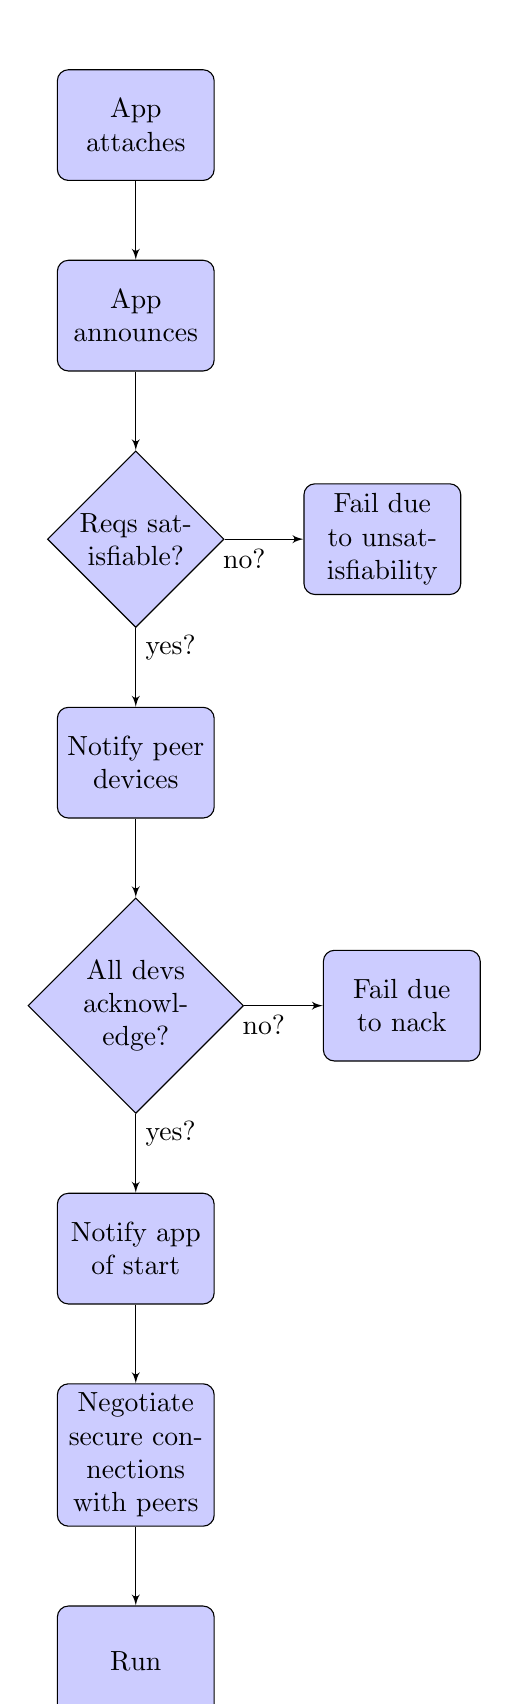
\begin{tikzpicture}
        [
            line/.style = {
                draw,
                -latex'
            },
            block/.style = {
                rectangle,
                draw,
                fill=blue!20,
                text width=5em,
                text centered,
                rounded corners,
                minimum height=4em
            },
            decision/.style = {
                diamond,
                draw,
                fill=blue!20,
                text width=4.5em,
                text badly centered,
                inner sep=0pt
            }
        ]

        \node[block] (attach) {App attaches};
        \node[block,below=of attach] (announce) {App announces};
        \node[decision,below=of announce] (satisfiable) {Reqs satisfiable?};
        \node[block,right=of satisfiable] (unsatisfied) {Fail due to unsatisfiability};
        \node[block,below=of satisfiable] (askpeers) {Notify peer devices};
        \node[decision,below=of askpeers] (ack) {All devs acknowledge?};
        \node[block,right=of ack] (nack) {Fail due to nack};
        \node[block,below=of ack] (start) {Notify app of start};
        \node[block,below=of start] (negotiate) {Negotiate secure connections with peers};
        \node[block,below=of negotiate] (run) {Run};

        \path[line] (attach) -- (announce);
        \path[line] (announce) -- (satisfiable);
        \path[line] (satisfiable) -- node[near start,below] {no?} (unsatisfied);
        \path[line] (satisfiable) -- node[near start,right] {yes?} (askpeers);
        \path[line] (askpeers) -- (ack);
        \path[line] (ack) -- node[near start,below] {no?} (nack);
        \path[line] (ack) -- node[near start,right] {yes?} (start);
        \path[line] (start) -- (negotiate);
        \path[line] (negotiate) -- (run);
    \end{tikzpicture}

    \caption{Connecting an app}
\end{figure}

\subsection{Low-level protocol}

The low-level protocol determines how the actual packets sent between client and server are constructed.
It specifies a common format independent of the actual transport layer that is used to guarantee a common understanding of how to handle incoming bytes.
The protocol is currently designed to be used over either TCP or UDP but should be generic enough to be used for other transport layers.
We will concentrate on describing design choices based on TCP and UDP transport layours only, though.

The major difference between TCP and UDP is that TCP is stream based and UDP is packet based.
This means that UDP packages have their size attached to the package itself, so it is guaranteed that when receiving a single package over UDP we know package boundaries and thus can split incoming packages by these boundaries.
On TCP this is not true, though, so we need to design a package format which is able to specify package boundaries so the client is able to determine a unit.

The initial design simply prefixed every single package with an unencrypted package length fixed to four bytes in network byte order.
This allowed the client to initially receive four bytes, convert these to host byte order and subsequently receive the amount of bytes specified.
While easy to implement this has several disadvantages.

The most obvious disadvantage is that the package length was always transmitted unencrypted.
It would have been possible to always encrypt the length with an attached message authentication code so that it is impossible to tamper with the length, but this would require us to always add the additional overhead of the attached MAC.
But even if the length was encrypted the attacker could be able to guess contents of sent packages based on their package lengths only.
Especially the package length packages will always be of fixed size universally known to all clients such that they are able to fetch the exact amount of bytes required to obtain the length of the follow package data.
Due to this shortcoming it becomes much easier for the adversary to do traffic analysis based on package sizes.

Another minor disadvantage is based on performance.
Assumed a single big package is sent over the wire.
With the simple case of an encrypted connection between client and server the client would be required to fetch the whole package before he is able to actually decrypt its content.
As the network layer is slow compared to doing computations on locally available data it would be of advantage to decrypt arriving data while waiting for subsequent bytes to arrive.
This would decrease the overall time required to receive and decrypt a big package.

To fix these problems the implementation resorts to packages of a fixed length.
The initial fixed-length package is prefixed with the overall length of the assembled package.
If the overall length exceeds the length of the remaining bytes of the first fixed length package, then the complete package is assembled by concatenating the first package all subsequent packages until the desired length is received.
The package length is only encoded in the first split package and all split packages are encrypted on their own.
The last package is right-padded with zeroes until it is as big as the other packages.

The following example demonstrates the package format for unencrypted packages.
We assume a fixed length package size of 64 bytes.
If a party now wishes to transfer a complete package of 80 bytes the complete package will get split into two partial packets.
The first package would be prefixed with four bytes of the complete package length and filled with the initial $64 - 4 = 60$ bytes.
The second package is filled with the remaining $80 - 60 = 20$ bytes and right-padded with $64 - 20 = 44$ zeroes.
Figure \ref{fig:unencrypted-package-format} visualizes both package contents.

\begin{figure}
    \center

    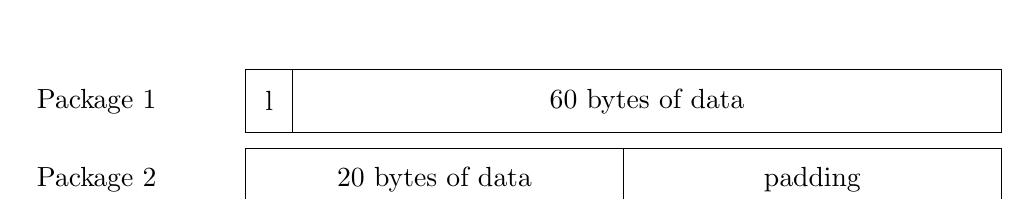
\begin{tikzpicture}[
            every node/.style={ minimum width=6mm, minimum height=8mm },
            start chain=1 going right,
            start chain=2 going right,
            node distance=-0.15mm
        ]

        \node[draw, on chain=1, minimum width=6mm] {l};
        \node[draw, on chain=1, minimum width=90mm] {60 bytes of data};
        \node[left=1cm of 1-1] {Package 1};

        \node[draw, on chain=2, minimum width=48mm, below=1cm of 1-1.west, anchor = west] {20 bytes of data};
        \node[draw, on chain=2, minimum width=48mm] {padding};
        \node[left=1cm of 2-1] {Package 2};
    \end{tikzpicture}

    \caption{Unencrypted package format}
    \label{fig:unencrypted-package-format}
\end{figure}

The second example (see figure \ref{fig:encrypted-package-format}) demonstrates how encrypted packages work.
In contrast to unencrypted packages there is an additional message authentication code attached to each split package which is now assumed to be 16 bytes long.

\begin{figure}
    \center

    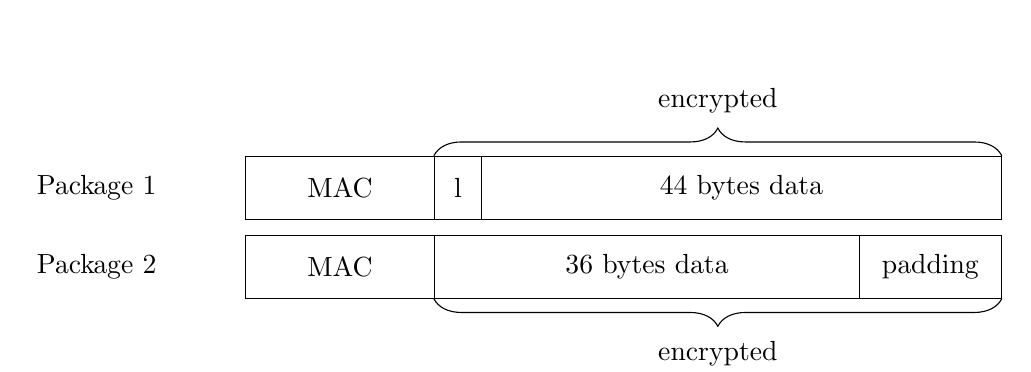
\begin{tikzpicture}[
            every node/.style={ minimum width=6mm, minimum height=8mm },
            start chain=1 going right,
            start chain=2 going right,
            node distance=-0.15mm
        ]

        \node[draw, on chain=1, minimum width=24mm] {MAC};
        \node[draw, on chain=1, minimum width=6mm ] {l};
        \node[draw, on chain=1, minimum width=66mm] {44 bytes data};
        \node[left=1cm of 1-1] {Package 1};

        \node[draw, on chain=2, minimum width=24mm, below=1cm of 1-1.west, anchor = west] {MAC};
        \node[draw, on chain=2, minimum width=54mm] {36 bytes data};
        \node[draw, on chain=2, minimum width=18mm] {padding};
        \node[left=1cm of 2-1] {Package 2};

        \draw [decorate,decoration={brace,amplitude=10pt}] (1-2.north west) -- (1-3.north east) node[midway,yshift=7mm] {encrypted};
        \draw [decorate,decoration={brace,amplitude=10pt,mirror}] (2-2.south west) -- (2-3.south east) node[midway,yshift=-7mm] {encrypted};
    \end{tikzpicture}

    \caption{Encrypted package format}
    \label{fig:encrypted-package-format}
\end{figure}

On the client side to process the split packages we will fetch the initial fixed-size package.
If the connection is encrypted, we will check the decrypt the message and verify the message authentication code.
Now we inspect the first four bytes to gain knowledge about the total package length -- if it exceeds the amount of bytes sent in the initial message, we will receive, verify and decrypt all following packages until all bytes are received.
Finally, we concatenate all content together to obtain the complete package.

\subsection{Connection establishment}

\begin{figure}
    \centering

    \begin{sequencediagram}
        \newthread{c}{Client (Verify$_c$, Sign$_c$)}
        \newthread[4]{s}{Server (VerifyS, SignS)}

        \begin{call}{c}{GenerateKeypair()}{c}{(EmphPriv$_c$, EmphPub$_c$)}
            \postlevel
        \end{call}

        \postlevel

        \begin{messcall}{c}{SignC(VerifyC || EmphPubC), VerifyC, EmphPubC}{s}
        \end{messcall}

        \begin{call}{s}{VerifyC(Signature)}{s}{}
            \postlevel
        \end{call}

        \begin{call}{s}{GenerateKeypair()}{s}{(EmphPriv$_s$, EmphPub$_s$)}
            \postlevel
        \end{call}

        \begin{messcall}{s}{SignS(EmphPubS || EmphPubC), EmphPubS, EmphPubC}{c}
        \end{messcall}

        \begin{call}{c}{VerifyS(Signature)}{c}{}
            \postlevel
        \end{call}

        \begin{messcall}{c}{SignC(EmphPubS || EmphPubC), EmphPubS, EmphPubC}{s}
        \end{messcall}

        \begin{call}{s}{VerifyC(Signature)}{s}{}
            \postlevel
        \end{call}

        \begin{call}{c}{GenSessionKey(EmphPubS, EmphPrivC)}{c}{Key}
            \postlevel
        \end{call}

        \begin{call}{s}{GenSessionKey(EmphPubC, EmphPrivS}{s}{Key}
            \postlevel
        \end{call}

        \postlevel

        \begin{messcall}{c}{ConnectionType}{s}
            \postlevel
        \end{messcall}
    \end{sequencediagram}

    \caption{Connection establishment}
    \label{fig:connection-establishment}
\end{figure}

% TODO: define functions

\subsection{Protocol}

\subsubsection{Discovery}

Device discovery is the process of discovering previously unknown services in a certain subnet.
To achieve the discovery, a client has to query all possible addresses in this subnet and subsequently await responses from servers.
This can easily be achieved with UDP multicast, that is we send a message to the multicast address of the subnet.
As UDP is port based it is mandatory that we choose a well-known port in advance to the protocol as otherwise it would be impossible to bootstrap the initial communication.

There are two major distinctions on how service discovery can be achieved: a client- and a service-driven approach.
The service-driven is based on the service periodically sending an announce message to the multicast address, thereby notifying possibly listening clients of the availability of a certain service.

The client-driven approach on the other side lets the client query the subnet for existing services by announcing that it wants to know about available services.
Every service that is listening and that receives this request will then answer the client and announce its presence.

Both methods have their own merit.
Periodic announcements of the service conceal the intent of clients to discover local services as they are not directly involved in the process of finding services.
They have the disadvantage of additional overhead, though, as we regularly have to announce our service.
While this might not be problematic when only few services are available in a certain subnet it may become unwieldy when hundreds of services are present.

This disadvantage is mitigated by the probing approach by clients that want to discover nearby services.
Just how important this is gets particularly clear when we consider the process how users want to start interacting with a certain service.
Assume that a user starts up his mobile phone with our app with the intent to start using a certain service.
With the periodic probing approach the user will in the worst case have to wait for the whole time span between two announcements of the service he wants to connect to.
Depending on how this timeout was chosen this may be an uncomfortably long time.
As users are generally uncomfortable with doing nothing for a rather long time (CITATION NEEDED) they might simply stop waiting and just scrap their plan.

When we directly probe the subnet for available services instead the response times will in the mean case be much less than in the other case.
That is the delay of services popping up is only based on latency and processing time of both service and client.
As a consequence we have chosen the probing approach.\\

The initial exchange between a client and service which have never seen each other before is somewhat problematic, as in general we cannot establish the authenticity of either one.
To accomodate for this we distinguish between undirected (see figure \ref{fig:service-discovery}) and directed service discovery(see figure \ref{fig:directed-service-discovery}).
While the undirected discovery protocol is unauthenticated we are able to improve the situation for directed service discovery in certain cases.

Through a sidechannel we are able to retrieve additional data about a service we want to connect to.
As described by McCune et al. \cite{mccune2005seeing} we can establish additional trust amongst other things by scanning a QR code that is either printed on the case of the service or, further improving the trust level, by dynamically displaying a QR code on the screen.
This is particularly interesting in the case where we want to connect to a display service.
Upon notifying the service in a certain out-of-band way (e.g. by pressing a certain button on the display) it will generate a QR code and display it on the screen.
The client can subsequently scan the code and in such a way retrieve information like the public key and address of the display.
As soon as we have obtained data through this side channel we are able to verify authenticity of the service we are communicating with, assuming the side channel has not been compromised.

Let us now consider the actual discovery protocol.

\begin{figure}[H]
    \centering

    \begin{sequencediagram}
        \newinst{s1}{Service 1}
        \newthread[4]{c}{Client}
        \newinst[4]{s2}{Service 2}

        \mess{c}{Discover}{s1}
        \prelevel
        \mess{c}{Discover}{s2}

        \postlevel

        \mess{s1}{Announce}{c}
        \mess{s2}{Announce}{c}
    \end{sequencediagram}

    \caption{Service Discovery}
    \label{fig:undirected-service-discovery}
\end{figure}

We assume both client and service own a long term key pair $(pk_c, sk_c)$ and $(pk_s, sk_s)$, respectively, that is used for establishing their own identity.
The initial \emph{Discover} message contains a protocol version, port and the public key of the client.

The version is required as future iterations on the protocol may lead to incompatibilities between different versions of the software stack that is in use on both client and service.
It is of utmost importance to check those versions for both parties to avoid running into incompatibilities that may cause the protocol to seemingly work while in fact it is broken in a subtle way.

When the service receives a UDP message the originating address is recorded in this message.
When we want to respond to that message, though, we are not able to do so without also knowing which port to send that response to, as UDP is a connection-less protocol.
As such we include a listing port inside the initial message that will be used by the service to send the response message.

Last we also include the client's long term public key to establish the client's identity and which will be used in future exchanges to encrypt further messages.
The whole message is then signed by the client and sent to the service.\\

On the receiving side we first unpack the message to retrieve version, port and public key.
With the public key and the message's tag we are now able to verify the integrity of the received package.
Obviously, though, we are not able to say anything about the authenticity about it as it could have been intercepted by a malicious third party, exchanging the message tag and public key.

After establishing message integrity the service will now compare the client's version to its own version and only proceed if he is able to correctly service that version.
He will then assemble a response package containing its own version, name, available local services and its public key.

It is possible for a single server to announce multiple services.
Those services may be distinguished by the port they are listenging at.
Instead of announcing multiple service types at a single port, which would then require multiplexing requests to their respective service and thus introduce additional complexity, each service has its own port which will later be used to connect to that service.

% TODO: encrypt message with public key?
The server will now again generate a message tag and send both message and tag encrypted with the public key of the client to the client's listening port that has been previously announced.

In contrast to the indirected service discovery, there is only one significant difference in the directed service discovery.
As we have previously obtained public key data of the server we want to talk to we are already able to use its key to encrypt the first message.
That is instead of sending $m \| t$ in the fisrt step, we send $\text{Enc}_{pk_s}(m \| t)$.
Like this it is impossible to tamper with the first message in such a way that the receiver retrieves a valid message with invalid key data.

All subsequent steps remain unchanged.

\subsubsection{Query}

\begin{figure}[H]
    \centering

    \begin{sequencediagram}
        \newthread{c}{Client}
        \newinst[8]{s}{Server}

        \begin{messcall}{c}{InitiateConnection()}{s}
            \postlevel
            \begin{call}{c}{Query()}{s}{Service description}
            \end{call}
        \end{messcall}

    \end{sequencediagram}
    \caption{Query Diagram}
\end{figure}

\subsubsection{Session Initiation}

\begin{align*}
    \text{capability} \coloneqq pk_s(\text{sessionid}, \text{parameters})
\end{align*}

\begin{figure}[H]
    \centering

    \begin{sequencediagram}
        \newthread{c}{Client}
        \newinst[8]{s}{Server}

        \begin{messcall}{c}{InitiateConnection()}{s}
            \postlevel
            \begin{call}{c}{InitiateSession(parameters)}{s}{Session Capability}
            \end{call}
        \end{messcall}

        \postlevel

        \begin{messcall}{c}{InitiateConnection()}{s}
            \postlevel
            \begin{messcall}{c}{Connect(session capability)}{s}
            \end{messcall}
        \end{messcall}

        \prelevel
    \end{sequencediagram}
    \caption{Direct Connect}
\end{figure}

\subsection{Services}

\subsubsection{Capability Service}

\begin{figure}[H]
    \centering

    \begin{sequencediagram}
        \newthread{r}{Requester r}
        \newinst[2]{e}{Entity e}
        \newinst[2]{s}{Service s}
        \newinst[2]{c}{Capability Server}

        \mess{e}{Register}{c}
        \postlevel

        \begin{call}{r}{Request(e, s, params)}{c}{Service Session}
            \postlevel
            \begin{call}{c}{Ask(r, s, params)}{e}{Service Session}
                \postlevel
                \begin{call}{e}{Initiate(params)}{s}{Service Session}
                \end{call}
                \postlevel
            \end{call}
            \postlevel
        \end{call}

        \postlevel

        \begin{messcall}{r}{Start}{s}
            \postlevel
        \end{messcall}

        \prelevel
    \end{sequencediagram}
    \caption{Capability Request}
\end{figure}

\subsubsection{Invoke Service}

\begin{figure}[H]
    \centering

    \begin{sequencediagram}
        \newthread{c}{Client}
        \newinst[4]{s}{Service}
        \newinst[4]{i}{Invoker}

        \begin{call}{c}{Initiate(Parameters)}{s}{Service Session}
            \begin{call}{s}{CreateSession()}{s}{Session}
            \end{call}
        \end{call}

        \postlevel

        \begin{call}{c}{Initiate(ServiceSession)}{i}{Invoker Session}
            \begin{call}{i}{CreateSession()}{i}{Session}
            \end{call}
        \end{call}
        \postlevel

        \begin{messcall}{c}{Start}{i}
            \begin{messcall}{i}{Start}{s}
                \postlevel
            \end{messcall}
            \prelevel
        \end{messcall}
        \prelevel
    \end{sequencediagram}

    \caption{Invoke Service}
\end{figure}

\subsection{xpra Service}

\begin{figure}[H]
    \centering

    \begin{sequencediagram}
        \newinst{x}{Xpra server}
        \newthread[4]{c}{Client}
        \newinst[4]{s}{Display service}

        \begin{call}{c}{Start(port)}{x}{instance}
        \end{call}

        \postlevel

        \begin{messcall}{c}{InitiateConnection()}{s}
            \postlevel
            \begin{call}{c}{Request(xpra-port)}{s}{session}
            \end{call}
        \end{messcall}

        \postlevel

        \begin{messcall}{c}{InitiateConnection()}{s}
            \postlevel
            \begin{messcall}{c}{Connect(session)}{s}
            \end{messcall}

            \postlevel

            \begin{messcall}{s}{Tunneled data exchange}{x}
                \postlevel
            \end{messcall}
            \prelevel
            \prelevel
            \prelevel
            \begin{messcall}{x}{}{s}
            \end{messcall}
        \end{messcall}
    \end{sequencediagram}

    \caption{Xpra Service}
\end{figure}

\subsection{Notes}

\begin{itemize}
    \item host has graphic server
    \item only knows about window extents, not contents due to encryption
    \item initially gets all keyboard/mouse inputs
    \item upon mouse enter inside a window, notifies mouse server of window extents
    \item mouse server keeps track of relative mouse position, notifies server upon exit of extents
    \item window server registers shortcuts that are required for window changing
    \item shortcuts may NEVER be rebound by client applications

    \item you can attach and reattach apps to other devices without any problems!!!
    \item overlay in server manager when app is connected and reqs are not fulfilled
    \item one container may run multiple apps
        \begin{itemize}
            \item clustering based on security level
        \end{itemize}
\end{itemize}

% vim: ft=tex tw=0

    \section{Drivers}

% vim: ft=tex tw=0

    \section{Matchmaking}

% vim: ft=tex tw=0

    \section{Implementation}

\subsection{Benchmarking}

\subsubsection{Package length}

\begin{figure}[t]
    \centering

    \begin{subfigure}[t]{0.4\textwidth}
        \resizebox*{!}{0.9\textwidth}
        {
            \begin{tikzpicture}
                \begin{axis}[ylabel=Throughput (in MB/s),ymax=200,xmode=log,xlabel=Block length (in bytes)]
                    \addplot table [x=pkglen,y=tpenc, col sep=comma,discard if not={datalen}{256}] {data/bench.csv};
                    \addlegendentry{0ms latency}

                    \addplot table [x=pkglen,y=tpenc, col sep=comma,discard if not={datalen}{256}] {data/bench-2ms.csv};
                    \addlegendentry{2ms latency}

                    \addplot table [x=pkglen,y=tpenc, col sep=comma,discard if not={datalen}{256}] {data/bench-20ms.csv};
                    \addlegendentry{20ms latency}
                \end{axis}
            \end{tikzpicture}
        }
        \caption{256 bytes of data}
    \end{subfigure}
    \hspace{2em}
    \begin{subfigure}[t]{0.4\textwidth}
        \resizebox*{!}{0.9\textwidth}
        {
            \begin{tikzpicture}
                \begin{axis}[ylabel=Throughput (in MB/s),ymax=400,xmode=log,xlabel=Block length (in bytes)]
                    \addplot table [x=pkglen,y=tpenc, col sep=comma,discard if not={datalen}{1024}] {data/bench.csv};
                    \addlegendentry{0ms latency}

                    \addplot table [x=pkglen,y=tpenc, col sep=comma,discard if not={datalen}{1024}] {data/bench-2ms.csv};
                    \addlegendentry{2ms latency}

                    \addplot table [x=pkglen,y=tpenc, col sep=comma,discard if not={datalen}{1024}] {data/bench-20ms.csv};
                    \addlegendentry{20ms latency}
                \end{axis}
            \end{tikzpicture}
        }
        \caption{1 kilobyte of data}
    \end{subfigure}

    \vspace{1em}

    \begin{subfigure}[t]{0.4\textwidth}
        \resizebox*{!}{0.9\textwidth}
        {
            \begin{tikzpicture}
                \begin{axis}[ylabel=Throughput (in MB/s),ymax=650,xmode=log,xlabel=Block length (in bytes)]
                    \addplot table [x=pkglen,y=tpenc, col sep=comma,discard if not={datalen}{102400}] {data/bench.csv};
                    \addlegendentry{0ms latency}

                    \addplot table [x=pkglen,y=tpenc, col sep=comma,discard if not={datalen}{102400}] {data/bench-2ms.csv};
                    \addlegendentry{2ms latency}

                    \addplot table [x=pkglen,y=tpenc, col sep=comma,discard if not={datalen}{102400}] {data/bench-20ms.csv};
                    \addlegendentry{20ms latency}
                \end{axis}
            \end{tikzpicture}
        }
        \caption{100 kilobytes of data}
    \end{subfigure}
    \hspace{2em}
    \begin{subfigure}[t]{0.4\textwidth}
        \resizebox*{!}{0.9\textwidth}
        {
            \begin{tikzpicture}
                \begin{axis}[ylabel=Throughput (in MB/s),ymax=650,xmode=log,xlabel=Block length (in bytes)]
                    \addplot table [x=pkglen,y=tpenc, col sep=comma,discard if not={datalen}{10240000}] {data/bench.csv};
                    \addlegendentry{0ms latency}

                    \addplot table [x=pkglen,y=tpenc, col sep=comma,discard if not={datalen}{10240000}] {data/bench-2ms.csv};
                    \addlegendentry{2ms latency}

                    \addplot table [x=pkglen,y=tpenc, col sep=comma,discard if not={datalen}{10240000}] {data/bench-20ms.csv};
                    \addlegendentry{20ms latency}
                \end{axis}
            \end{tikzpicture}
        }
        \caption{10 megabyte of data}
    \end{subfigure}

    \caption{Sending data with different block lengths}
\end{figure}

\begin{figure}
    \centering
    \begin{tikzpicture}
        \begin{axis}[ylabel=Time (in ms),ymax=2100,xlabel=Network latency (in ms)]
            \addplot table [x=latency,y=connect, col sep=comma] {data/latency.csv};
            \addlegendentry{Client}

            \addplot table [x=latency,y=await, col sep=comma] {data/latency.csv};
            \addlegendentry{Server}
        \end{axis}
    \end{tikzpicture}
    \caption{Connection latency}
\end{figure}

% vim: ft=tex tw=0


    \clearpage
    \nocite{*}
    \bibliography{resources/bibliography}
\end{document}

% vim: ft=tex tw=0
